%!TEX root = nextndnvideo-tr.tex
\section{prior work} % (fold)
\label{sec:comparison}
\begin{figure}%[htbp]
  \centering
  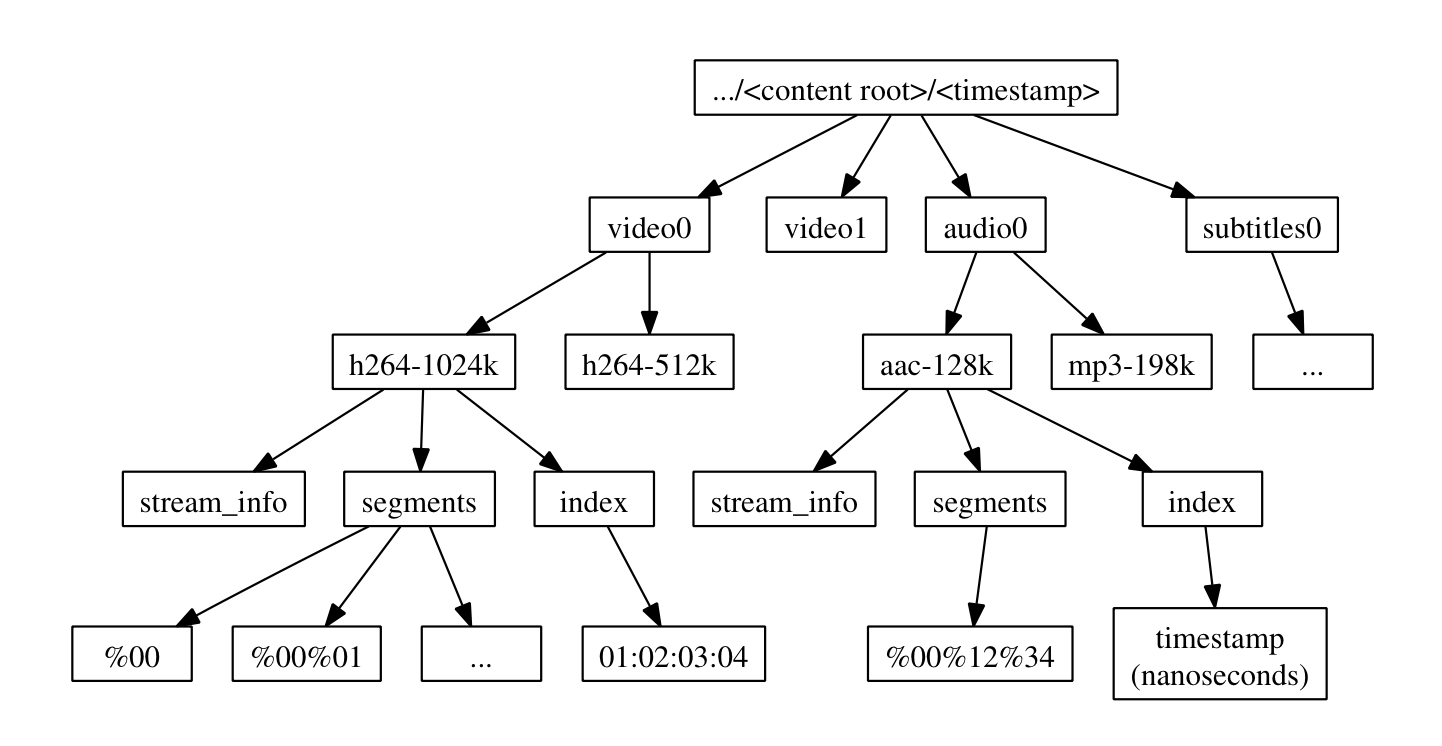
\includegraphics[scale=0.3]{ndnvideo_naming}
  \vspace{-0.3cm}
  \caption{Prior NDNVideo Naming Space}
  \label{fig:ndnvideo_naming}
  \vspace{-0.2cm}
\end{figure}

\begin{table*}[ht]	
	\centering
	\begin{tabular}{|c|c|c|c|}

	\hline
	             & NDNlive \& NDNtube                                      & NDNVideo                                  & NDN-RTC                   \\ \hline 
	Dependencies & \begin{tabular}[c]{@{}c@{}}ndn-cxx / NFD\\ Consumer / Producer API\end{tabular} & \begin{tabular}[c]{@{}c@{}}CCNx / CCNR \\ pyccn\end{tabular}  & ndnx / NFD\\ \hline
	Media Processing    & Gstreamer 1.x                                    & Gstreamer 0.1                             & WebRTC                            \\ \hline
	Framing      & video \& audio frames                                   & fixed segments                            & video \& audio frames                   \\ \hline
	Language     & c++                                                     & python                                    & c++                   \\ \hline
	\end{tabular}
	\caption{Comparison with NDNVideo and NDN-RTC}
	\label{table:comparison}
\end{table*}

NDNVideo provides live and pre-recorded video streaming over NDN using Gstreamer library for media processing and Repo for permanent storage~\cite{ndnvideo}. Since the new NFD does not support the previous packet format, this implementation of video streaming is now obsolete.

The major difference between NDNlive~/~NDNtube and NDNVideo is the organization of the video and audio content. In the NDNVideo, video or audio streams are chopped into fixed-size segments, which requires a special mapping between real playback time and segment numbers to keep video and audio synced, and support ``seek'' functionality (Figure~\ref{fig:ndnvideo_naming}). Fixed-size segmentation breaks the boundaries of frames (e.g. Application Data Units), which causes the inter-dependency between different frames leading to the problems inherent to TCP/IP such as Head-Of-Line (HOL) blocking.

In NDNlive and NDNtube, video and audio streams are chopped into frames. One frame may contain several segments. Since segmentation is provided by Consumer / Producer API, it is transparent for the application, which has to focus only at frame level. Since every frame has a unique name and is independent from any other frames, any missing frames do not affect other frames, which is highly beneficial for video streaming applications, especially for live streaming applications. For example, in NDNlive, if the previous frame can't be retrieved on time, the consumer can just skips it and continues with the next frame to keep the video streaming. 

NDN-RTC \cite{ndn-rtc} is a real-time video conferencing library, which was designed to provide an enduser experience similar to Skype or Google Hangouts. Just like NDNlive, it also fetch video and audio data frame by frame. But they are different in these aspects. Firstly, key frame and delta frame will have different namesapce in NDN-RTC, while we don't distinguish them in NDNlive implementation. Secondly, we use Consumer/Producer API to handle frame segmentation in producer side and retransmission and segments reassembling inside one frame in consumer side. NDN-RTC all do these by themselves. That is the obvious benefit which Consumer / Producer API brought to us. Thirdly, we all keep some outstanding interests requesting for segments which are ready to generate but not be generated yet to provide the low latency video and audio fetching. However, the way how we compute the number of outstanding interests and the way of pipelining frame fetching are all different. And the libraries we use to deal with the media are also different. What's more, NDN-RTC is a library, while NDNlive is an application. We design to provide an application that one producer produces video streaming and multi-consumers consume the same video stream. But they provide a library to support multi-users sharing a video conference. It means that NDN-RTC supports multi-producers and multi-consumers. We just differ from the design aim.

Table~\ref{table:comparison} illustrates other significant differences such as library dependencies and versions, and programming languages.


